% This text is proprietary.
% It's a part of presentation made by myself.
% It may not used commercial.
% The noncommercial use such as private and study is free
% Sep. 2005 
% Author: Sascha Frank 
% University Freiburg 
% www.informatik.uni-freiburg.de/~frank/
%
% additional usepackage{beamerthemeshadow} is used
%  
%  \beamersetuncovermixins{\opaqueness<1>{25}}{\opaqueness<2->{15}}
%  with this the elements which were coming soon were only hinted
\documentclass{beamer}
%\usetheme{bars}
\usepackage{beamerthemeshadow}
\begin{document}
\title{Offline Handritting Word Recognition}  
\author{Thijs Kooi, Davide Modolo}
\date{\today} 

\frame{\titlepage} 

\frame{\frametitle{Table of contents}\tableofcontents} 

% SECTION: OVERVIEW OF THE PROJECT
\section{Overview}

\frame{
\begin{beamerboxesrounded}{}
\centering Overview of the Project
\end{beamerboxesrounded}
}
\subsection{General}
\frame{\frametitle{Off-line handwriting recognition}  
\begin{itemize}
\item It involves the automatic conversion of text in an image into letter codes which are usable within computer and text-processing applications
\item Off-line handwriting recognition is comparatively difficult, as different people have different handwriting styles

\begin{figure}
  \centering
    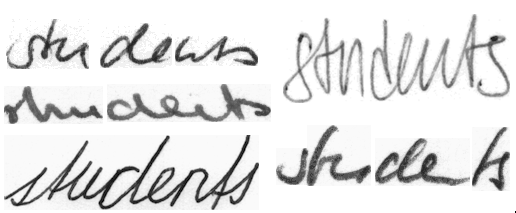
\includegraphics[width=0.5 \textwidth]{Images/studs.png}
   \caption{'Students' written by different authors}
   \label{fig:student}
\end{figure}
\end{itemize}
}

\frame{\frametitle{Our AI Project}
A lot of research has been done over the past years.\vspace{\baselineskip}

We explored the topic and implemented a full pipeline for the task.
The research touched different fields:
\begin{itemize}
\item Data Collection
\item Image Processing
\item Features extraction 
\item Machine Learning 
\item Word Recognition
\end{itemize}
}

\subsection{Dataset}
\frame{\frametitle{Dataset}
The IAM Handwriting Database 3.0\footnote{http://www.iam.unibe.ch/fki/databases/iam-handwriting-database}  \vspace{\baselineskip}

\begin{itemize}
%\item It contains forms of handwritten English text which can be used to train and test handwritten text recognizers and to perform writer identification and verification experiments.
\item Unconstrained handwritten text (scanned at a resolution of 300dpi and saved as PNG images with 256 gray levels) 
\item 1'539 pages of scanned text of 657 writers
\item 13'353 isolated and labeled text lines
\item 115'320 isolated and labeled words
\end{itemize}
}

\frame{\frametitle{Example of a page of scanned text}  
\begin{figure}
  \centering
    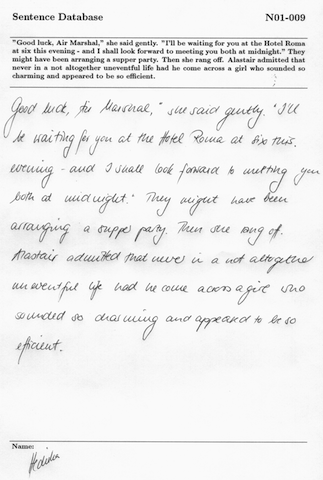
\includegraphics[width=0.5\textwidth]{Images/database.png}
   \caption{Example of page of scanned text}
   \label{fig:dataset}
\end{figure}
}


%SECTION: IMPLEMENTATION DETAILS
\section{Implementation Details}
\frame{
\begin{beamerboxesrounded}{}
\centering Implementation Details
\end{beamerboxesrounded}
}

\subsection{Pipeline}
\frame{\frametitle{Pipeline}  
\begin{figure}
  \centering
    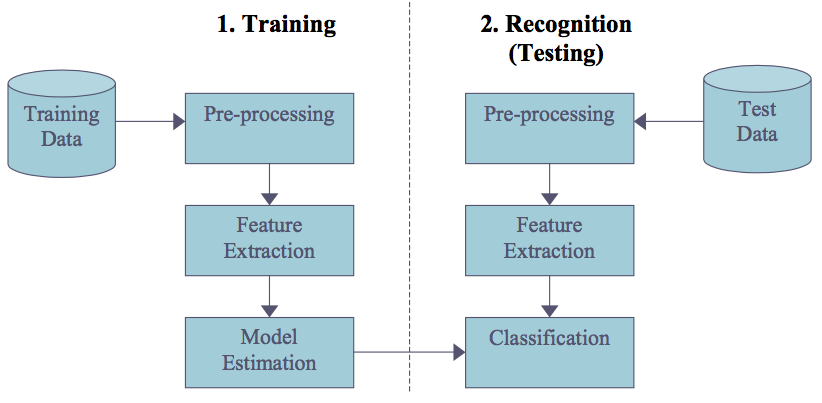
\includegraphics[width=1.02 \textwidth]{Images/pipeline.png}
   \caption{Pipeline of a word recognition system}
   \label{fig:pipeline}
\end{figure}
}

\subsection{Pre-Processing}
\frame{
\begin{beamerboxesrounded}{Implementation Details}
\centering Pre-Processing
\end{beamerboxesrounded}
}

\frame{\frametitle{Pre-processing}  
\begin{figure}
  \centering
    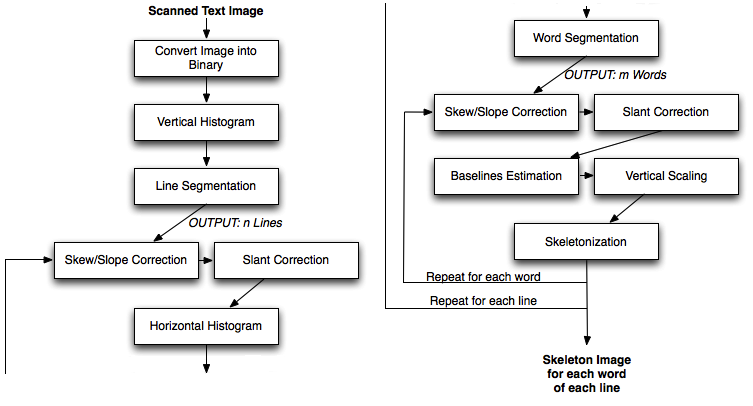
\includegraphics[width=1\textwidth]{Images/pipelinePP.png}
   \caption{Pipeline for the pre-processing/normalization step}
   \label{fig:pipeline}
\end{figure}
}



\frame{\frametitle{Line Segmentation}  
\begin{figure}
  \centering
    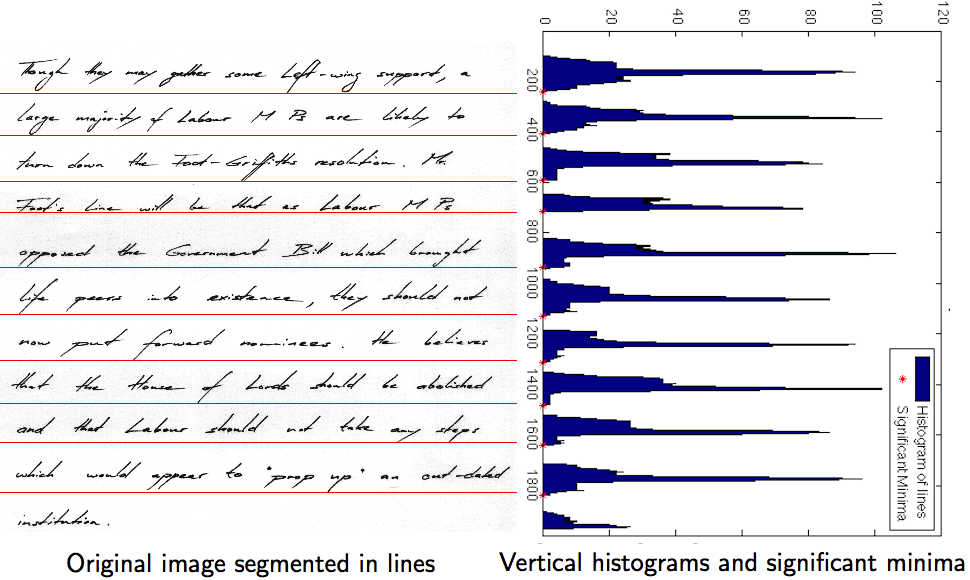
\includegraphics[width=0.93 \textwidth]{Images/line_segmentation.png}
   \caption{Example of line segmentation}
   \label{fig:lineSegm}
\end{figure}
}


\frame{\frametitle{Skew and Slope Correction}  
\begin{figure}
  \centering
    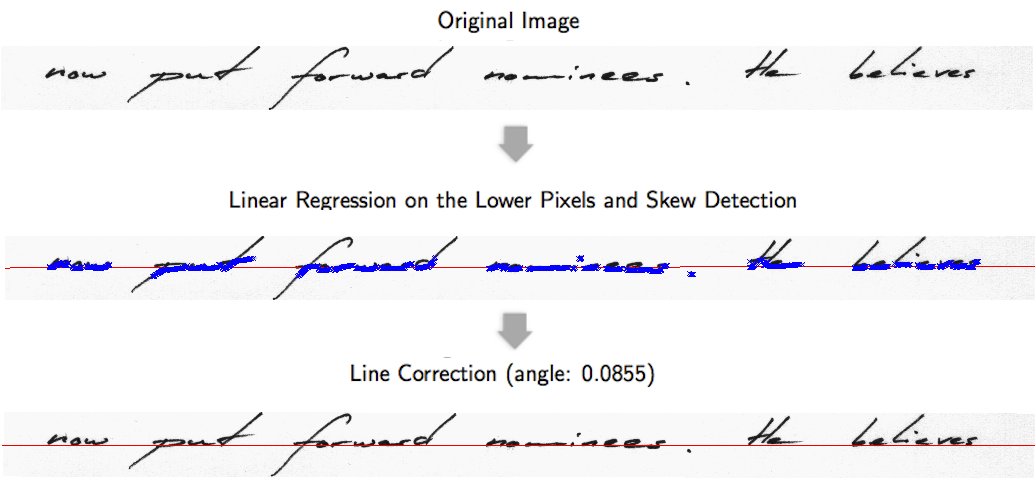
\includegraphics[width=1.0 \textwidth]{Images/skew.png}
   \caption{Skew detection and correction pipeline}
   \label{fig:skew}
\end{figure}
}


\frame{\frametitle{Slant Correction}  
\begin{figure}
  \centering
    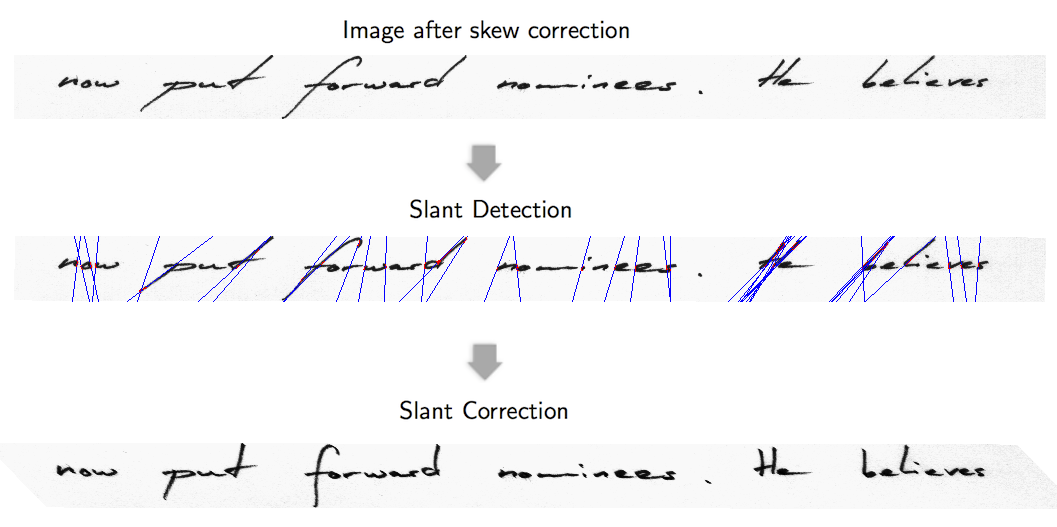
\includegraphics[width=1 \textwidth]{Images/slant.png}
   \caption{Slant detection and correction pipeline}
   \label{fig:slant}
\end{figure}
}

\frame{\frametitle{Word segmentation}
\begin{figure}
  \centering
    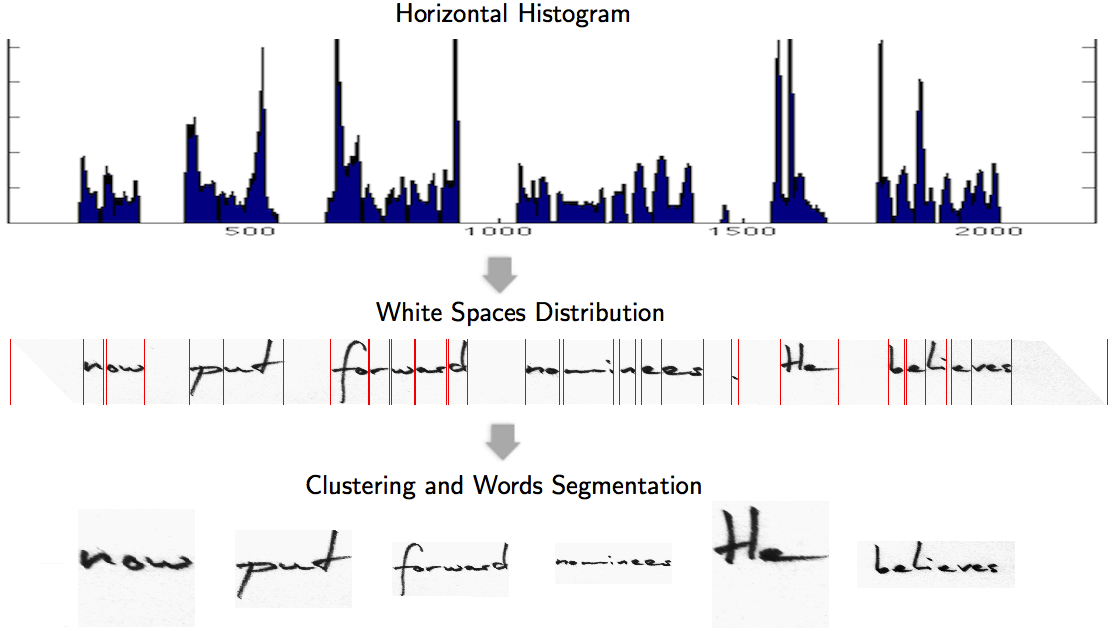
\includegraphics[width=1.0 \textwidth]{Images/word_segmentation.png}
   \label{fig:words_res}
\end{figure}
}  

\frame{\frametitle{Vertical Scaling}
}  

\frame{\frametitle{Skeletonization}
}  

\frame{\frametitle{Remembering the entire pipeline....}
 \begin{beamerboxesrounded}{}
\centering \bf{Why repeating skew and slant correction twice?}
\end{beamerboxesrounded}
\begin{figure}
  \centering
    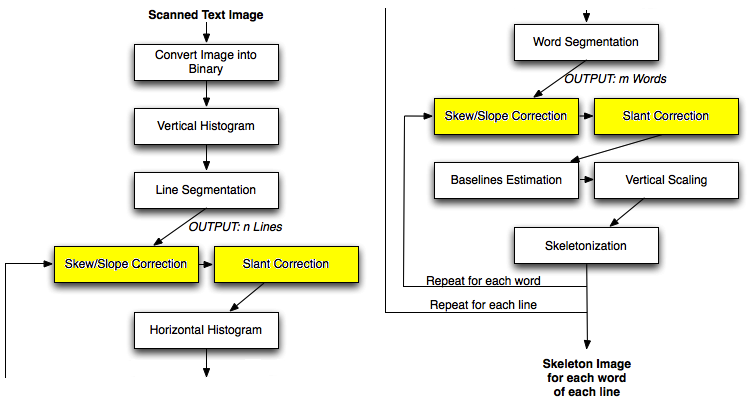
\includegraphics[width=1\textwidth]{Images/pipelinePPex.png}
   \label{fig:pipeline}
\end{figure}
}  

\frame{\frametitle{Because....}
\begin{figure}
  \centering
    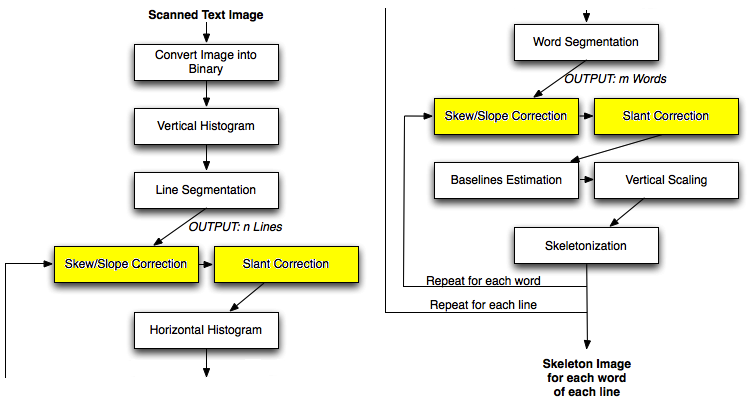
\includegraphics[width=1\textwidth]{Images/pipelinePPex.png}
   \label{fig:pipeline}
\end{figure}

}  





\subsection{Feature Extraction}
\frame{
\begin{beamerboxesrounded}{Implementation Details}
\centering Feature Extraction
\end{beamerboxesrounded}
}

\frame{\frametitle{Features}  
  We want to find features that minimise the within-class variability and maximise the between class variability. On top of this, the features should be robust againts distortions caused by different handwriting styles. Moreover, we want to find low dimensional featur vectors and would therefore like features to be highly descriptive.
  The selection of features depends both on the pre-processing and the classifier to use. If all characters are assumed to have the same oriention, we need rotation variant features to distinguish between for instance a 6 and a 9 and a b and an p, etc.
  
}

\subsection{Hidden-Markov Model}
\frame{\frametitle{HMM}
  \begin{itemize}
  \item A set of $N$ states $S = (s_{1}, s_{2}, \ldots, s_{N})$, where the state of the system at time $t$ is denoted $q_{t}$
  \item A set of priors ${\bf \pi} = (\pi_{1}, \pi_{2}, \ldots, \pi_{N})$, providing the probability $P(q_{1} = s_{i})$.
  \item A transition function ${\bf A}$, where $a_{ij} = P(q_{t+1} = s_{j} | q_{t} = s_{i})$. 
  \item An observation function ${\bf B}$, mapping each observation at every state to a probability $b_{i}({\bf o}_{t}) = P({\bf o}_{t} | q_{t} = s_{i}, \lambda)$, where $\lambda$ denotes the model parameters.
  \end{itemize}
  The model is trained to estimate the posterior probability $P({\bf O}|\lambda)$ of an observation sequence ${\bf O}$, with $D$-dimensional observation vectors ${\bf o}_{t} = (o_{1},o_{2},\ldots,o_{D})$.
}

\frame{\frametitle{HMM}  

  \begin{figure}
  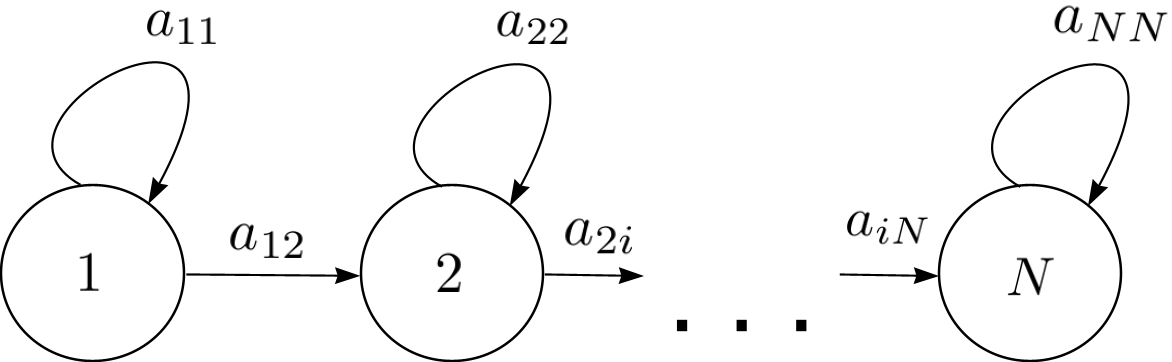
\includegraphics{hmm.jpg} 
  \caption{Left-to-right HMM with N states}
  \end{figure}

}

\frame{\frametitle{Main problems in an HMM}
  \begin{enumerate}
 \item The probability of an observation sequence, given the model, $P({\bf O}|\lambda)$.
 \item The most likely parameters of the model $\lambda^* = \max P(X|\lambda)$, given a training set of $M$ observation sequences $X = ({\bf O}_{1}, {\bf O}_{2}, \ldots, {\bf O}_{M} )$.
  \item The most likely state sequence, underlying a given observation sequence and the model, $Q^* = \max P(Q|{\bf O},\lambda)$.
\end{enumerate}
}

\frame{\frametitle{Main problems in an HMM}
  \begin{enumerate}
 \item The probability of an observation sequence, given the model, $P({\bf O}|\lambda)$.
 \begin{beamerboxesrounded}{}
   Sum-product algorithm: forward-backward algorithm
\end{beamerboxesrounded}
	
 \item The most likely parameters of the model $\lambda^* = \max P(X|\lambda)$, given a training set of $M$ observation sequences $X = ({\bf O}_{1}, {\bf O}_{2}, \ldots, {\bf O}_{M} )$.
  \begin{beamerboxesrounded}{}
  EM-algorithm: Baum-Welch reestimation
\end{beamerboxesrounded}
      
\item The most likely state sequence, underlying a given observation sequence and the model, $Q^* = \max P(Q|{\bf O},\lambda)$.
  \begin{beamerboxesrounded}{}
  Dynamic programming: Viterbi algorithm
\end{beamerboxesrounded}

\end{enumerate}
}

\frame{\frametitle{Forward probability}
\begin{columns}
 
\column{1.5in}
\[
 \alpha_{t}(i) \equiv
\]
\[
  P(o_{1},o_{2},\ldots, o_{t}| q_{t} = s_{i}, \lambda) = 
\]
\begin{equation}
 \label{forwardProbability}
\displaystyle \Big [ \sum_{j=1}^{N}  \alpha_{t-1}(j) a_{ij} \Big ] b_{j}(o_{t})
\end{equation}
\column{2in}
  \begin{figure}
  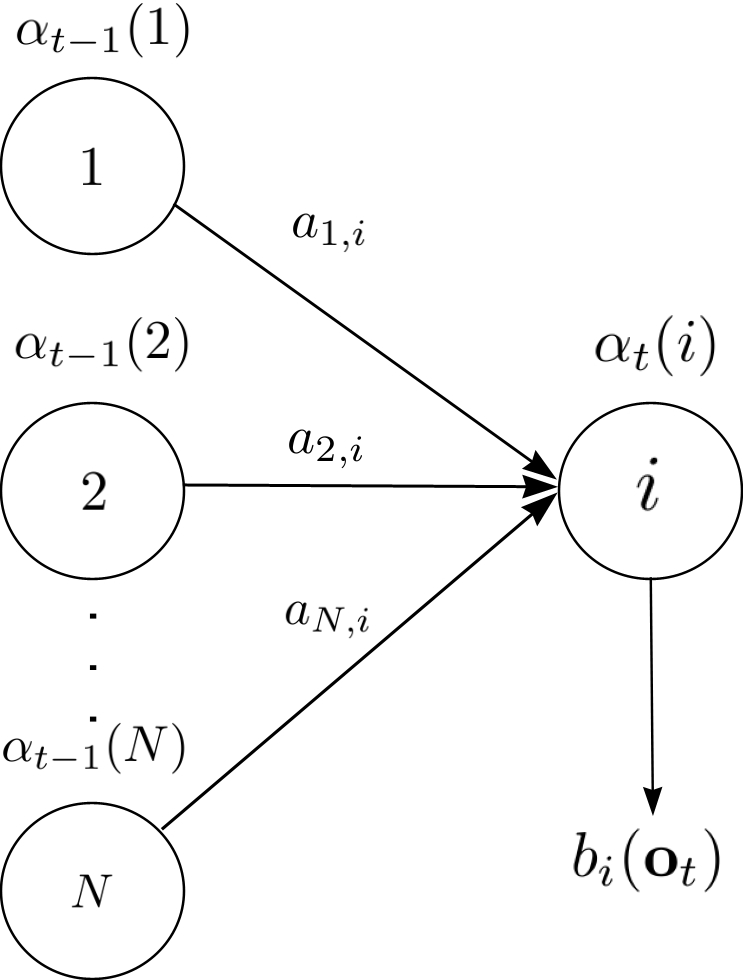
\includegraphics[width=0.8\textwidth]{forward2.jpg}
  \caption{Computation of forward probability}
  \end{figure}

\end{columns}

}

\frame{\frametitle{Forward probability}
\begin{columns}
 
\column{1.5in}
\[
 \alpha_{t}(i) \equiv
\]
\[
  P(o_{1},o_{2},\ldots, o_{t}| q_{t} = s_{i}, \lambda) = 
\]
\begin{equation}
 \label{forwardProbability}
\displaystyle \Big [ \sum_{j=1}^{N}  \alpha_{t-1}(j) a_{ij} \Big ] b_{j}(o_{t})
\end{equation}
\begin{equation}
 P({\bf O| \lambda}) = \displaystyle \sum_{i=1}^{N} \alpha_{T}(i)
\end{equation}
Problem 1 solved.
\column{2in}
  \begin{figure}
  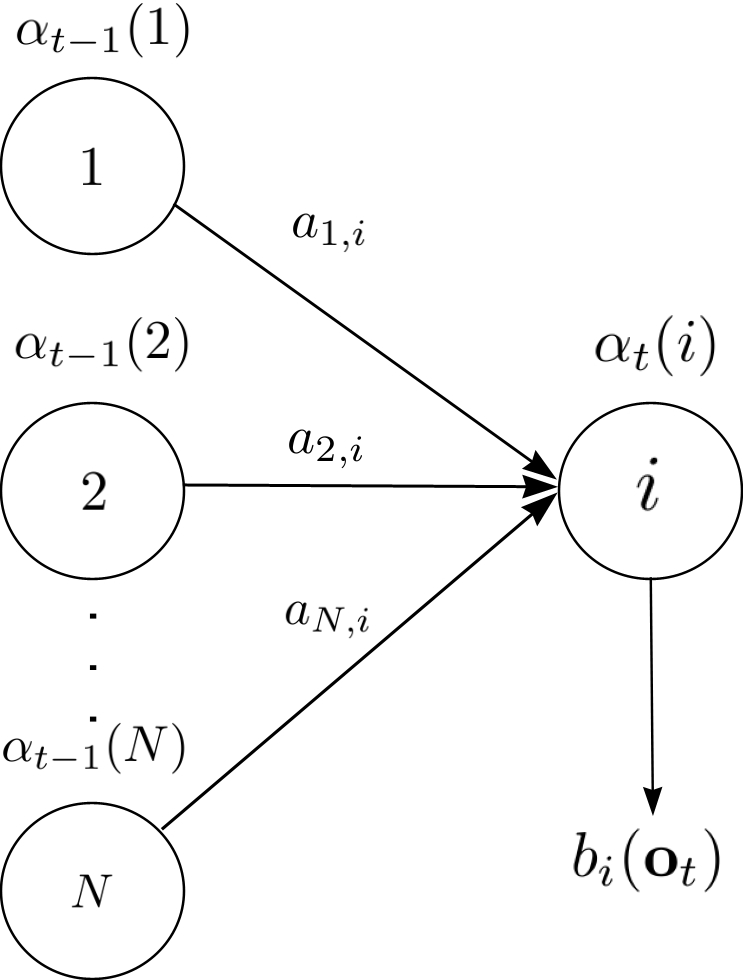
\includegraphics[width=0.8\textwidth]{forward2.jpg}
  \caption{Computation of forward probability}
  \end{figure}

\end{columns}

}

\frame{\frametitle{Updating the parameters}
  The forward-backward algorithm also commes with a backward probability:\\
 \[
  \beta_{t}(j) \equiv P(o_{t+1},o_{t+2},\ldots, o_{T}| q_{t} = s_{j}, \lambda) = 
\]
\begin{equation}
 \label{backwardProbability}
\displaystyle \sum_{i=1}^{N} a_{ij} b_{i}(o_{t+1}) \beta_{i}(o_{t+1})
\end{equation}
With this we can define the probability of being in a state at a timestep as:
\begin{equation}
 \gamma_{t}(i) \equiv (P({\bf O}|\lambda))^{-1} \alpha_{t}(i)\beta_{t}(i) 
\end{equation}
Where normalisation constant $P({\bf O}|\lambda) = \sum_{j=1}^{N} \alpha_{t}(i)\beta_{t}(i) = \sum_{j=1}^{N} \alpha_{T}(j)$.

}

\frame{\frametitle{Updating the parameters}

  Comparison with GMM:
\begin{table}
 \begin{tabular}{|l| p{3.5cm} | p{3.5cm} |}\hline
  Model:		&	{\bf GMM}		&	{\bf HMM}\\\hline
  Model parameters:	& $\lambda = \pi, \mu, \Sigma$	&	$\lambda = \pi, {\bf A}, {\bf B}$\\
  Hyper parameters:	&	Number of components	&	Topology (states, transitions)\\
  Observed variables:	&	Data points		&	Observations\\
  Latent variables:	&	Priors of a component	&	State sequence\\\hline
 \end{tabular}
\end{table}

}

\frame{\frametitle{Updating parameters}

% \begin{columns}

% \column{1.5in}
% Model:\\
% Model parameters:\\
% Observed variables:\\
% Latent variables:\\
% E-step:\\
% M-step:\\
% 
% \column{1.5in}
% {\bf GMM}\\
% $\lambda = \pi, \mu, \Sigma$\\
% Data points\\
% Priors of a component\\
% Estimate the probability of a component, given the data and current parameters.\\
% Maximise $\pi$, $\mu$ and $\Sigma$.
% 
% \column{1.5in}
% {\bf HMM}\\
% $\lambda = \pi, {\bf A}, {\bf B}$\\
% Observation sequence\\
% State sequence\\
% Estimate the probability of being in a state at a timestep and the probability of transfering from a state to another state.\\
% Maximise $\pi$, ${\bf A}$ and ${\bf B}$.
% \end{columns}

\begin{table}
 \begin{tabular}{|l| p{3.5cm} | p{3.5cm} |}\hline
  Model:		&	{\bf GMM}		&	{\bf HMM}\\\hline
  E-step:		&	Estimate the probability of a component, given the data and current parameters. 
	& Estimate the probability of being in a state at a timestep and the probability of transfering from a state to another state.\\
  M-step:		& Maximise $\pi$, $\mu$ and $\Sigma$.	&	Maximise $\pi$, ${\bf A}$ and ${\bf B}$\\\hline
 \end{tabular}
\end{table}


}



\frame{\frametitle{Problems we ran into}
Consider the following observation:
  \[
   {\bf O} = \begin{pmatrix}
        -1 & 0\\
	2 & 0\\
	1 & 0\\
	-2 & 0\\
       \end{pmatrix}
  \]
}

\frame{\frametitle{Problems we ran into}
  Singularities. Consider the following observation:
  \[
   {\bf O} = \begin{pmatrix}
        -1 & 0\\
	2 & 0\\
	1 & 0\\
	-2 & 0\\
       \end{pmatrix}
  \]
  \[
   \Sigma = \begin{pmatrix}
        3\frac{1}{3} & 0\\
	0 & 0\\
       \end{pmatrix}
  \]
}
\frame{\frametitle{Problems we ran into}
 Singularities
  \[
   {\bf O} = \begin{pmatrix}
        -1 & 0\\
	2 & 0\\
	1 & 0\\
	-2 & 0\\
       \end{pmatrix}
  \]
  \[
   \Sigma = \begin{pmatrix}
        3\frac{1}{3} & 0\\
	0 & 0\\
       \end{pmatrix}
  \]
\[
 |\Sigma| = 0
\]

\begin{beamerboxesrounded}{}
\centering   Possible solution: Add some random noise.
\end{beamerboxesrounded}

}
\frame{\frametitle{Problems we ran into}
 Singularities
  \[
   {\bf O} = \begin{pmatrix}
        -1 & 0\\
	2 & 0\\
	1 & 0\\
	-2 & 0\\
       \end{pmatrix}
  \]
  \[
   \Sigma = \begin{pmatrix}
        3\frac{1}{3} & 0\\
	0 & 0\\
       \end{pmatrix}
  \]
  -> Add some random noise, also to prevent variance from collapsing.
}

\frame{\frametitle{Problems we ran into}

Short words have less likelihood.\\
Harder to recognise, more subject to writer variations.

tried to solve this by using MOG.

}
\section{Results}
\frame{\frametitle{Results}  
blabla
}



\section{Conclusions}
\frame{\frametitle{Conclusions}  
blabla
}



%\section{Pre-Processing} 
%\frame{\frametitle{Title} 
%Each frame should have a title.
%}
%
%\frame{ 
%Without title somethink is missing. 
%}
%
%
%\section{Feature Extraction} 
%\subsection{Lists I}
%\frame{\frametitle{unnumbered lists}
%\begin{itemize}
%\item Introduction to  \LaTeX  
%\item Course 2 
%\item Termpapers and presentations with \LaTeX 
%\item Beamer class
%\end{itemize} 
%}
%
%\frame{\frametitle{lists with pause}
%\begin{itemize}
%\item Introduction to  \LaTeX \pause 
%\item Course 2 \pause 
%\item Termpapers and presentations with \LaTeX \pause 
%\item Beamer class
%\end{itemize} 
%}
%
%\subsection{Lists II}
%\frame{\frametitle{numbered lists}
%\begin{enumerate}
%\item Introduction to  \LaTeX  
%\item Course 2 
%\item Termpapers and presentations with \LaTeX 
%\item Beamer class
%\end{enumerate}
%}
%\frame{\frametitle{numbered lists with pause}
%\begin{enumerate}
%\item Introduction to  \LaTeX \pause 
%\item Course 2 \pause 
%\item Termpapers and presentations with \LaTeX \pause 
%\item Beamer class
%\end{enumerate}
%}
%
%\section{Section no.3} 
%\subsection{Tables}
%\frame{\frametitle{Tables}
%\begin{tabular}{|c|c|c|}
%\hline
%\textbf{Date} & \textbf{Instructor} & \textbf{Title} \\
%\hline
%WS 04/05 & Sascha Frank & First steps with  \LaTeX  \\
%\hline
%SS 05 & Sascha Frank & \LaTeX \ Course serial \\
%\hline
%\end{tabular}}
%
%
%\frame{\frametitle{Tables with pause}
%\begin{tabular}{c c c}
%A & B & C \\ 
%\pause 
%1 & 2 & 3 \\  
%\pause 
%A & B & C \\ 
%\end{tabular} }
%
%
\section{Section no. 4}
\subsection{blocs}
\frame{\frametitle{blocs}

\begin{block}{title of the bloc}
bloc text
\end{block}

\begin{exampleblock}{title of the bloc}
bloc text
\end{exampleblock}


\begin{alertblock}{title of the bloc}
bloc text
\end{alertblock}
}
\end{document}


